%% LyX 2.0.5.1 created this file.  For more info, see http://www.lyx.org/.
%% Do not edit unless you really know what you are doing.
\documentclass[english,a4paper,english,czech,12pt]{article}
\usepackage[utf8]{inputenc}
\usepackage{babel}
\usepackage{url}
\usepackage{amstext}
\usepackage{amssymb}
\usepackage{graphicx}
\usepackage[unicode=true,
 bookmarks=true,bookmarksnumbered=false,bookmarksopen=false,
 breaklinks=false,pdfborder={0 0 1},backref=false,colorlinks=false]
 {hyperref}
\hypersetup{pdftitle={MyslenkyTermodynamiky},
 pdfauthor={Martin Holi Holecek}}

\makeatletter
%%%%%%%%%%%%%%%%%%%%%%%%%%%%%% User specified LaTeX commands.
\usepackage{amsthm,amsmath,amssymb,amscd,mathrsfs,url}
%\usepackage[czech]{babel}
\usepackage{verbatim}
\usepackage{showkeys}
\usepackage{xcolor}
\usepackage{stackengine}
\usepackage{lipsum}
\usepackage{comment}
%%\usepackage{MNsymbol} NIKDY!
\usepackage{graphicx}
\usepackage{tikz}
\usepackage{marginnote}
\usepackage{esint}
\setlength\textwidth{145mm}
\setlength\textheight{247mm}
\newcommand{\opdiv}{\mathop{\mathrm{div}}}
\newcommand{\oprot}{\mathop{\mathrm{rot}}}

\makeatother

\begin{document}

\title{Souhrn myšlenek z termodynamiky}

\maketitle
Teplo je neuspořádaný pohyb částic systému.

Termodynamický stav je přesný popis zkoumaného objektu. Pozorované
veličiny jsou nutně středované (přez fluktuace).

Makrostav je termodynamický stav, je realizován velkým počtem mikrostavů
(které mají ekvivalentní hodnotu termodynamických veličin).

Rozdělovací funkce, střední hodnoty, fluktuující částice, poissnovo
rozdělení.


\paragraph*{Nultá věta}

Systém je v termodynamické rovnováze, pokud jsou pozorovatelné veličiny
nezávislé na čase.

Širší formulace - ...pozorovatelné veličiny středované přez fluktuace
nezávislé ...

Když se systém vyvíjí - nerovnovážný.

Systém není v rovnováze, pokud v něm tečou toky (částic). Např pro
elektronický obvod ano, ale zdroj musí být součástí experimentu.

Systém je v ustáleném stavu, když jsou toky konstantní.

Termodynamickou rovnováhu fixují okrajové podmínky a vnitřní energie.


\paragraph*{Přesuny energie a vratnost}
\begin{itemize}
\item Konáním práce $\delta W$. Vratný děj - práci použiju k vrácení se
k předchozímu stavu.
\item Tokem tepla $\delta Q$. Limitně vratný děj - se zvyšujícím se počtem
rezervoárů se dá přiblížit blíž původnímu stavu předáváním tepla.
\item Disipativní prací (tření). Nevratný. Konáním $\delta W$ se získá
rovnou $\delta Q$.
\end{itemize}
V reálu každý děj obsahuje trochu toho dissipativního.

Adiabatický proces. Teplo přechází vždy mezi nějakými tělesy.

Stavová veličina - veličina termodynamického stavu. Nestavová veličina
- veličina nějakého děje.


\paragraph*{První termodynamická věta $1VTD$}

\[
dE=\delta Q+\delta W
\]


Princip zachování energie. Systém energii ztrácí/získává pouze konáním
práce nebo tokem tepla, pro konání práce platí:

\[
\delta W=-pdV
\]



\paragraph*{Druhá termodynamická věta (tvar s přechodem tepla)}

Neexistuje proces, při kterém by přecházelo teplo z tělesa chladnějšího
na teplejší, aniž by zbytek světa zůstal nezměněn.


\paragraph*{Kvantová mechanika}

Vlastní stavy a měřitelné hodnoty jsou vlastní vektory a vlastní čísla.

Rozlišitelnsot a nerozlišitelnost částic.

V jednom stavu pouze jeden fermion. Bosonů libovolně. Dva fermiony
je jeden boson. Fermion má spin.

Degenerace (více stavů na jednu hodnotu veličiny).

Stern Gerlach - měření spinu v jiném směru zresetuje předchozí měření
a znovu se změří náhoda. Spin změní operátor co nekomutuje.

Konečný počet stavů, nicméně velký.

Kvazispojitost stavů. Velmi malý rozdíl hodnot mezi sousedními stavy,
rozdíly lze aproximovat derivací proložené spojité funkce.


\paragraph*{Hustota stavů}

\[
g(E)=\frac{dN}{dE}
\]


Kolik stavů se vejde do intervalu energie.


\paragraph*{Gibbsův statistický soubor}

Protože měřní ovlivněno fluktuacemi, středujeme přez statistický soubor.
Buď musím opakovat měření, anebo začínám s vícero systémy ve stejném
makrostavu (liší se pouze mikrostavy).


\paragraph*{Klasifikace statistických souborů z hlediska podmínek}
\begin{itemize}
\item Mikrokanonický $\delta E=0\,\&\,\delta N=0$
\item Kanonický $\delta E\neq0\,\&\,\delta N=0$
\item Grandkanonický $\delta E\neq0\,\&\,\delta N\neq0$
\end{itemize}

\paragraph*{Stirlingův vzorec}

$\ln N!\simeq N(\ln N-1)$

$N!\simeq(\frac{N}{e})^{N}\sqrt{2\pi N}$


\paragraph*{Princip stejné rovnovážné pravděpodobnosti}

Systém je v termodynamické rovnováze $\iff$ jsou všechny pravděpodobnosti
všech dovolených konfigurací stejné.

Jinak se systém vyvíjí. (Dovolené konfigurace jsou samovolně, fluktuacemi
dosažitelné mikrostavy.)

V rovnováze platí následující vzoreček

\[
p_{i}=\frac{1}{g(E_{i})}\delta(E_{i}-E_{0})
\]


$\delta$ je neurčitost - mikroskopická. Makroskopicky je jedna energie
ale vícero mikrostavů co jí realizujou.

Důkaz - v rovnováze platí $\forall i:\, p_{i}=\frac{1}{\delta(E)\, N}\delta(E)=\frac{1}{N}$.
Platí protože všechny pravděpodobnosti stavů jsou v rovnováze stejné.

Rovnost platí, protože $N=\int_{E_{0}}^{E_{0}+\delta(E)}g(E)dE$,
kde predpokladame, ze $\delta(E)$ je tak male, ze v intervalu lze
$g(E)$ polozit konstantni. I kdyz $g(E)$ rychle roste, vzdy lze
vzit $\delta(E)$ tak male, aby to platilo.


\paragraph*{Fázový prostor $\Phi$}

$N$ částic ve $3D$ má hybnosti a polohy, tzn $3N+3N=6N$ je dimenze
fázového prostoru. Každá konfigurace je pak bodem ve fázovém prostoru.

To je pojem klasické fyziky, přidáme princip neurčitosti:

Měřením (polohy) částici uzavřeme do potenciálové jámy, kde schrodingerova
rovnice a okrajové podmínky přesně řeknou, že lze naměřit místo původní
přesné hybnosti pouze hybnosti v diskrétních hodnotách $p_{n}=\frac{\pm\pi\hbar n}{\delta x}$.

Chyba v měření (je interval mezi sousedními $n$, resp. $p_{n}$)
nám tedy říká kolik fázového objemu zabírá jedna částice $\Delta p\delta x=2\pi\hbar$.
To je objem jedné rozlišitelné částice.

Počet rozlišitelných konfigurací v jedné dimenzi objemu $p_{M}L$
je $n=\frac{2p_{M}L}{2\pi\hbar}$.

Jedna $3D$ částice má tedy fázový objem $(2\pi\hbar)^{3}$, $N$
částic ve $3D$ (tj. orig. má $3D$, fázový prostor má dimenzi $6N$
) má objem jednoho stavu $(2\pi\hbar)^{3N}$.

Počet rozlišitelných konfigurací tedy závisí na přiděleném objemu
takto: $\Gamma=\frac{\delta\Phi}{(2\pi\hbar)^{3N}}$.


\paragraph*{Teplota}

Odvození z hustoty stavů $g(E)$ a dvou systémů s celkovým počtem
stavů $g_{tot}\sim g_{A}(E_{A})g_{B}(E_{tot}-E_{A})$ ($\sim$ protože
nemusí souhlasit jednotky).

Pro logaritmus pak platí (konstanta z $\sim$ vymizí):

\[
\ln(g_{tot})=\ln(g_{A}(E_{A}))+\ln(g_{B}(E_{tot}-E_{A}))
\]


V extrému $0=dE_{A}+dE_{B}$ je derivace nulová:

\[
\frac{\partial\ln(g_{tot})}{\partial E}=\frac{\partial\ln(g_{A}(E_{A}))}{\partial E_{A}}-\frac{\partial\ln(g_{B}(E_{B}))}{\partial E_{B}}
\]


... a tedy se veličiny rovnají.

Pokud tedy zavedeme teplotu jako derivaci logaritmu počtu stavů, bude
automaticky veličinou charakterizující tok tepla od teplejšího ke
studenějšímu. Navíc díky provedenému výpočtu bude vidět, že systémy
budou v rovnováze, pokud budou mít stejnou teplotu. Tedy

\[
\frac{\partial\ln(g(E))}{\partial E}=\frac{1}{k_{B}T}=\beta
\]


... kde $T$ je teplota, $k_{B}$ je Boltzmannova konstanta, $\beta$
je chladnost. Vybudováno ze statistické fyziky, dle hustoty stavů.


\paragraph*{Clausiova formulace druhé věty termodynamické}

Teplo nemůže téct spontánně z tělesa chladnějšího na těleso teplejší.
Opak není vyloučen (fluktuace), ale statisticky je málo pravděpodobný.


\paragraph*{Boltzmannovo rozdělení a teplota malých systémů}

Teplota zavedená pro systémy s hustotou stavů, tj pouze pro makroskopické.
Zobecnění na systémy s malým počtem stavů ($S$) následující úvahou
s rezervoárem.

Chceme pro malý systém $S$ znát pravděpodobnosti, s jakými nabývá
různých hladin energie v závislosti na dané teplotě (rezervoáru) -
$p(E_{i})$.

Nechť je v kontaktu se systémem $S$ rezerovár $R$, dohromady v termodynamické
rovnováze. Mají tedy stejnou zadanou teplotu $T$.

Rezervoár splňuje, díky známé rovnici z definice teploty, pro $g$:

\[
\frac{\partial\ln(g(E_{R}))}{\partial E_{R}}=\frac{1}{k_{B}T}
\]


... tedy vyjádřená $g$ bude exponenciální funkcí teploty (protože
předchozí řádek je diferencíální rovnice pro $g$):

\[
g_{R}\sim e^{E_{R}/(k_{B}T)}
\]


Počet stavů systému $S$ a $R$ dohromady je $1\cdot g_{R}$, protože
systém $S$ je malý, jednu energii nese pouze jeden stav. Navíc pravděpodobnost,
že systém nese energii $E_{i}$ lze vyjádřit rozdílem od společné
energie obou systémů dohromady $E_{tot}=E_{R}+E_{i}$:

Jinak - jaká je pravděpodobnost, že systém $S$ má energii $E_{i}$?
Přesně taková, že $R$ má energii $E_{tot}-E_{i}$, protože hustota
stavů celku $R+S$ je stejná jako hustota stavů $R$ (protože malý
systém $S$ má pouze $1$ stav).

\[
p(E_{i})\sim1\cdot g_{R}(E_{tot}-E_{i})\sim e^{\frac{-E_{i}}{k_{B}T}}
\]


Druhou vlnovku dostaneme dosazením $g_{R}\sim e^{E_{tot}-E_{i}/(k_{B}T)}$,
kde dosazená $E_{tot}$ se schová do konstanty ve vlnovce $\sim$.

Vlnovky se zbavíme požadavkem na normování pravděpodobnosti, dostame
Boltzmannovo rozdělení:

\[
p_{i}=p(E_{i})=\frac{e^{\frac{-E_{i}}{k_{B}T}}}{\sum_{j}e^{\frac{-E_{j}}{k_{B}T}}}
\]



\paragraph*{Stavová/partiční suma/funkce}

Normovací konstanta se standarně značí $z=\sum_{j}e^{\frac{-E_{j}}{k_{B}T}}$,
``stavová/partiční suma/funkce\char`\"{}. Lze z ní spočíst jiné veličiny,
např:

\[
E=\sum_{i}p_{i}E_{i}=-\frac{\partial}{\partial\beta}\ln z
\]



\paragraph*{Nerovnovážné systémy a mistrovská rovnice}

Vývoj systému znamená vývoj pravděpodobností $p_{i}(t)$ nabývání
energetických hladin ($E_{i}$). Nutno říct, že energetické hladiny
se nemění a závisí na vnějších a okrajových podmíkách.

\[
\frac{dp_{i}}{dt}=\sum_{j}(P_{ij}p_{j}-P_{ji}p_{i})
\]


...tzn kolik stavů přejde za čas do stavu $i$, mínus kolik se jich
vrací. $P_{ij}$ je rychlost přechodu stavů.


\subparagraph*{Fermiho zlaté pravidlo}

Z kvantové mechaniky platí $P_{ij}=P_{ji}$.

Vytknutím z rovnice vývoje systému, pomocí tohoto faktu, získáme kinetickou/řídící/mistrovskou
rovnici.

\[
\frac{dp_{i}}{dt}=\sum_{j}P_{ij}(p_{j}-p_{i})
\]


Díky tomu je splněn princip stejné rovnovážné pravděpodobnosti. Mj.
přináší časovou nevratnost.


\paragraph*{Objem fázového prostoru}

Fázový prostor o dimenzi $6N$ s celkovou energií $\leq E$ pro částice
v objemu $V$ má objem 

\[
\Phi(E)=\int_{V\times\{\leq E\}}\, d^{3}\mu_{1}...d^{3}\mu_{N}\cdot d^{3}p_{1}...d^{3}p_{N}
\]


...což je objem krychle (za prostor) krát objem koule (za hybnosti
$\sum p_{i}^{2}/(2m)\leq E$):

\[
\Phi(E)=V^{N}\frac{\pi^{3N/2}(2mE)^{3N/2}}{\Gamma(3N/2+1)}
\]


Rozlišitelnou část fázoprostoru $\Phi_{D}(E)$ spočteme pomocí úvahy,
že libovolná permutace -vzájemná záměna- částic neovlivní pozici konfigurace
ve fázovém prostoru, tedy $\Phi_{D}(E)=\Phi(E)/N!$.

Dosazením a použitím stirlingova vzorečku k aproximaci jmenovatele
$\Gamma(3N/2+1)$ a $N!$, dostáváme:

\[
\Phi_{D}(E)=V^{N}\pi^{3N/2}(2mE)^{3N/2}\cdot(\frac{e}{N})^{N}(\frac{2e}{3N})^{3N/2}=(\frac{V}{N})^{N}(\frac{4\pi e^{5/3}m}{3})^{3N/2}(\frac{E}{N})^{3N/2}
\]


Což zavedením redukovaných veličin: $\epsilon=E/N,\, v=V/N$:

\[
\Phi_{D}(E)=v^{N}\epsilon^{3N/2}(\frac{4\pi e^{5/3}m}{3})^{3N/2}
\]


Dostali jsme objem rozlišitelných částic ideálního plynu pro zanedbané
energie interakcí a potenciální energii.


\subparagraph*{Změna objemu}

Malou změnou energie změníme řádově celý objem fázového prostoru,
je tedy silnou funkcí energie a většina stavů se nachází blízko slupky.


\subparagraph*{Počet rozlišitelných konfigurací}

Je objem rozlišitelných konfigurací fázového prostoru děleno objemem
jedné rozlišitelné konfigurace.

\[
\Gamma=\frac{\Phi_{D}(E,V)}{(2\pi\hbar)^{3N}}=(\frac{V}{N})^{N}(\frac{4e^{5/3}m}{3\pi\hbar^{2}N})^{3N/2}
\]


Lze vypočíst i z rozdělovací funkce $\Gamma=g(E)\Delta E$.


\paragraph*{Záporná teplota}

Nastává pro systémy, kde hustota stavů nabývá maximum na vrcholu kopečku.
Teplota $T$ pak přejde z $+\infty$ (levá strana kopečku) do $-\infty$
(pravá strana kopečku). Chladnost $\beta$ jen spojitě projde nulou.

Záporná teplota je pro energetičtější (teplejší) stavy, než kladná.
Dosáhnu jí tak, že budu přidávat energii, ale nikoliv teplem.

Tedy například pro soustavu spinů máme přesně hustotu stavů ve tvaru
kopečku. Soustavu spinů vyrovnáme polem rovnoběžně, ochladíme (zafixujeme)
a pak otočíme elektrické pole ... a spiny budou najednou ukazovat
proti poli a tak bude mít soustava skokově mnohem víc energie.


\paragraph*{Entropie $S$}

Zavedeme statisticky pomocí počtu rozlišitelných konfigurací. Lze
zavést termodynamicky (``existuje veličina''), což je ale nenázorné.

\[
S:=k_{B}\ln\Gamma
\]


...Boltzmannova definice pro mikrokanonický soubor. Pro případ kdy
všechny pravděpodobnosti jsou stejné ($p_{i}=1/\Gamma$), lze definovat
i s pomocí pravděpodobnosti:

\[
S:=-k_{B}\ln p_{i}
\]



\subparagraph*{Vlastnosti entropie}
\begin{itemize}
\item Aditivní (násobení počtu stavů přejde v logaritmu ve sčítání).
\item Nulová je pouze v jednom konkrétním stavu, to pouze pro absolutní
nulu.
\end{itemize}

\subparagraph*{Zobecnění - Boltzmann - Gibbsova definice:}

\[
S:=-k_{B}\sum_{i}p_{i}\ln p_{i}
\]


...vlastně střední hodnota z logaritmu. Definice je zobecnění, protože
pro mikrokanonický rovnovážný systém se vytkne logaritmus a suma sečte
na jedničku. Jako zobecněná je stále aditivní.

Pokud entropii přisoudíme jednotky $J\, K^{-1}$, budou v důsledku
souhlasit termodynamická teplota a jiné veličiny, které jsou závislé
na teplotě.


\paragraph*{Zákon růstu entropie - éta teorém}

Dosadíme mistrovskou rovnici $\frac{dp_{i}}{dt}=\sum_{j}P_{ij}(p_{j}-p_{i})$
do derivace entropie:

\[
dS:=-k_{B}\sum_{i}\dot{p_{i}}\ln p_{i}-k_{B}\sum_{i}p_{i}\dot{\ln p_{i}}=
\]


... druhý člen bude roven nule, protože $\sum_{i}p_{i}\dot{\ln p_{i}}=\sum_{i}\dot{p_{i}}=\dot{1}=0$
a do prvního dosadíme mistrovskou rovnici:

\[
=-k_{B}\sum_{i,j}P_{ij}(p_{j}-p_{i})\ln p_{i}=-\frac{1}{2}k_{B}\sum_{i,j}P_{ij}(p_{j}-p_{i})(\ln p_{i}-\ln p_{j})
\]


kde jsme díky symetrii $P_{ij}$ mohli přičíst totéž. Teď je totiž
vidět, že suma je vždy záporná - protože $p_{i}\geq p_{j}\iff\ln p_{i}\geq\ln p_{j}$.

Díky tomu je celá záležitost kladná $dS\geq0$ (nulová pouze pro stejné
pravděpodobnosti a/nebo pro reverzibilní procesy - jinak by v jednom
směru entropie mizela což by byl spor).


\paragraph*{Entropie a teplota}

Pokud máme hustotu stavů, pak $\Gamma=g(E)\Delta E$ (vlastnost rozdělovací
funkce). Proto lze aproximovat (v logaritmu jde zanedbat tím víc)

\[
S=k_{B}\ln(g(E)\Delta E)\simeq k_{B}\ln(g(E))
\]


A zderivujeme dle energie:

\[
(\frac{\partial S}{\partial E})_{V,N}=\frac{\partial k_{B}\ln(g(E))}{\partial E}=\frac{1}{T}
\]


(Stejný výsledek dostaneme, pokud máme $S(E,V)$ rozepsané do rovnosti
pro diferenciály.)


\paragraph*{Pozn. druhy entropie}

Kanonická entropie - pokud je pravděpodobnost dána Boltzmannovým rozdělením,
mluvím o kanonickém stavu. Kanonická entropie je dána vnějšími parametry
a jedním vnitřním ($T$ nebo $E$).

Konfigurační entropie - logaritus počtu defektů v pevné látce. (Přesná
krystalická mřížka pak má nulovou entropii).


\paragraph*{Vztahy mezi rovnovážnou entropií, teplem, prací}

Vyjdeme ze střední energie $E=\sum_{i}p_{i}E_{i}$

Rozepíšeme do diferenciálů

\[
dE=\sum_{i}p_{i}dE_{i}+\sum_{i}E_{i}dp_{i}
\]


Ukážeme, že jeden z těchto členů bude roven $\delta Q$ a druhý $\delta W$.

Protože vše bude rovnovážné a boltzmannovské, tak $E_{i}$ nesouvisí
s teplotou. $E_{i}$ jsou neměnné konstanty systému závisející na
okrajových podmínkách (např. objem).

Přidáváním tepla zvyšujeme jenom pravděpodobnosti dosažení vyšších
energetických hladin, tedy $\sum_{i}E_{i}\, dp_{i}=\delta Q$.

Z $1VTD$ plyne, že druhý člen je $\delta W$, nicméně lze to ukázat
i na základě faktu, že $dE$ se mění pouze změnou vnějších podmínek
(bez tepla), k tomu je potřeba síla. (Princip adiabatické invariance)

$\sum_{i}dE_{i}\, p_{i}=\delta W$

Nu a síla krát podmínka je práce, konkrétně třeba pro $V$: $\delta W=\sum_{i}p_{i}\frac{\partial E_{i}}{\partial V}\, dV=-p\, dV$
(protože z 1VTD je $p=-(\frac{\partial E_{i}}{\partial V})_{S}$).


\paragraph*{Vztah pro $dS$ a $\delta Q$ do $1VTD$}

\[
dS=d(-k_{B}\sum_{i}p_{i}\ln p_{i})=-k_{B}\sum_{i}dp_{i}\,\ln p_{i}-k_{B}\sum_{i}p_{i}\,1/p_{i}\, dp_{i}=
\]


...druhý člen vypadne, protože přehodíme sumu a diferenciál a zjistíme,
že se jedná o derivaci konstantní jedničky. Za $\ln p_{i}$ dosadíme
Boltzmannovské rozdělení $p_{i}=e^{-E_{i}/(k_{B}T)}/z$.

\[
=k_{B}\sum_{i}dp_{i}\, E_{i}/(k_{B}T)+k_{B}\sum_{i}dp_{i}\,\ln z=
\]


...z druhého členu vytkneme logaritmus, a opět záměnou sumy a diferenciálu
bude člen nulový. Na první člen použijeme rovnost $\sum_{i}E_{i}\, dp_{i}=\delta Q$.

\[
=1/T\,\sum_{i}dp_{i}\, E_{i}=\frac{\delta Q}{T}=dS
\]



\paragraph*{Diferenciální tvary}

Věta termodynamická ($1VTD$) pak lze psát v diferenciálním tvaru:

\[
dE=T\, dS-p\, dV
\]


Porovnáním této rovnice s rovností pro diferenciál funkce $E(S,V)$
dostaneme další možné vztahy:

\[
dE=(\frac{\partial E}{\partial S})_{V}\, dS+(\frac{\partial E}{\partial V})_{S}\, dV\,...\,(\frac{\partial E}{\partial S})_{V}=T,\,(\frac{\partial E}{\partial V})_{S}=p
\]


Navíc entropie je stavová, takže platí $0=\oint dS=\oint\frac{dQ}{T}$.

Mimochodem vztah co dává $T$ je podobný jako z části entropie a teplota
(ukazuje, že otočením derivací dostaneme $T^{-1}$).


\paragraph*{Populární rovnice většiny termodynamiky}

Předpokládejme $E(T,V)$ (jako v$1VTD$ ale s $T$ místo $S$ kvůli
budoucímu dosazování) a $S(T,V)$ ve stejných proměnných. Použijeme
rovnost pro diferenciály a upravíme $1VTD$ pro tvar $dS$:

\[
dS=(\frac{\partial S}{\partial T})_{V}\, dT+(\frac{\partial S}{\partial V})_{T}\, dV
\]


\[
dE=(\frac{\partial E}{\partial T})_{V}\, dT+(\frac{\partial E}{\partial V})_{T}\, dV
\]
\[
dS=\frac{1}{T}\, dE+\frac{p}{T}\, dV
\]


Uvážíme rovnost dvou vyjádření $dS$ - dle rovnosti pro diferenciál
(levá strana) a $1.VTD$ (pravá strana), kde dosadíme do $1VTD$ diferenciál
$E$ (dosazujeme proto, abychom dostali stejné diferenciály $dT$
a $dV$):

\[
(\frac{\partial S}{\partial T})_{V}\, dT+(\frac{\partial S}{\partial V})_{T}\, dV=dS=\frac{1}{T}\,(\frac{\partial E}{\partial T})_{V}\, dT+\frac{1}{T}\,((\frac{\partial E}{\partial V})_{T}+p)\, dV
\]


První mezivýsledek je rovnost koeficientů u diferenciálů $dT$, $dV$.
Tuhle rovnost použijeme dosazením do rovnosti druhých derivací:

\[
\frac{\partial^{2}S}{\partial V\partial T}=\frac{\partial^{2}S}{\partial T\partial V}
\]


\[
\frac{1}{T}\frac{\partial^{2}E}{\partial V\partial T}=-\frac{1}{T^{2}}\,((\frac{\partial E}{\partial V})_{T}+p)+\frac{1}{T}\,(\frac{\partial^{2}E}{\partial T\partial V}+(\frac{\partial p}{\partial T})_{V})
\]


A předpokládejme i záměnnost druhých derivací funkce $E$, díky tomu
dostaneme populární rovnici:

\[
(\frac{\partial E}{\partial V})_{T}=T\,(\frac{\partial p}{\partial T})_{V}-p
\]


Z rovnice pak pro jednoduché systémy platí ``pokud je tlak lineární
funkcí teploty, pak energie nezávisí na objemu\char`\"{}. Pro složitější
systémy máme diferenciální rovnici. V jiných případech lze získat
další vztahy dosazením za $p$ z $pV=Nk_{B}T$.


\paragraph*{Třetí věta termodynamická}

\[
T\rightarrow0\Rightarrow S\rightarrow0
\]


Netriviální výsledek klasické termodynamiky, nicméně pro náš způsob
odvození je jednoduché, protože pro $T=0$ máme jen jeden stav a $\ln1=0$.
Mimochodem pak i derivace entropie jsou nulové (kapacita a expanzní
koeficienty).

Navíc ground states nejsou degenerované, protože při nižších teplotách
se víc projevují síly zajišťující interakci.

Mimochodem, pomocí tohohle zákona lze měřit entropie přidáváním tepla,
sledováním teploty a integrací (samozřejmě ne od absolutní nuly, ale
třebas někde blízko).


\paragraph*{Rozdělovací funkce $f(E)$ energií}

Hustota pravděpodobnosti, že měřím právě energii $E$ se rovná hustotě
stavů nabývajících danou energii krát pravděpodobnosti nabytí této
energie.

\[
f(E)=g(E)\, p(E)
\]



\paragraph*{Fluktuace}

Jak široká je fukce $f(E)$? Jak se chová v okolí maxima? Vyšetřováním
derivací $\ln f$ (abychom pak mohli dosadit do Taylorova rozvoje):

\[
\frac{d\ln f}{dE}=\frac{d\ln g}{dE}+\frac{d\ln p}{dE}=\frac{1}{k_{B}T(E)}-\frac{1}{k_{B}T_{R}}=0
\]


Máme dvě teploty - rezervoár a systém, teplota systému osciluje s
energií, teplota rezervoáru určije pravděpodobnosti Boltzmannovským
rozdělením. Pro systém v kontaktu s rezervoárem jsme takhle zavetli
teplotu, která když se rovná teplotě rezervoáru, tak je stejná...
a proto je první derivace nulová.

Druhá derivace už bude značit fluktuaci:

\[
\frac{d^{2}\ln f}{dE^{2}}=-\frac{1}{k_{B}T^{2}}\frac{dT}{dE}=-\frac{1}{k_{B}T^{2}}\frac{1}{c}
\]


(což je též tepelná kapacita).

Taylor tedy vypadá takto:

\[
\ln f(E)=\ln f(E_{0})-\frac{1}{2k_{B}T^{2}}\frac{dT}{dE}(E-E_{0})^{2}+...
\]


Z čehož na okolí maxima funkce $f(E)$ v okolí maxima vypadá takto
$f=f_{0}\exp(-\frac{(E-E_{0})^{2}}{2k_{B}T^{2}c})$.

Funkce $f$ výrazně klesá, když $|E-E_{0}|\sim\sqrt{k_{B}\, T\, T\, c}$.
$k_{B}T$ je mikroskopická veličina, $T\, c$ makroskopická. Fluktuace
jdou s odmocninou.


\paragraph*{Ideální jednoatomový plyn a maxwellovo rozdělení rychlostí}

Cíl bude najít rozdělující funkci rychlostí (Maxwellovo rozdělení)
za předpokladu, že energie ideálního plynu je pouze kinetická energie.
Vezmeme nejprve rychlost pouze v jednom směru, $v_{x}$ a vezmeme
vztah z důkazu \char`\"{}Boltzmanova rozdělení a teplota malých systémů\char`\"{}
$(p(E_{i})\sim1\cdot g_{R}(E_{tot}-E_{i})\sim e^{\frac{-E_{i}}{k_{B}T}})$,
dostaneme

\[
p\sim e^{\frac{-mv_{x}^{2}}{2k_{B}T}}
\]


Rozdělovací funkci rychlosti dostaneme vynormováním:

\[
f(v_{x})=Ae^{\frac{-mv_{x}^{2}}{2k_{B}T}}
\]


Normovací konstantu $A$ spočteme pomocí vzorečku Gaussova integrálu:
\[
\int_{-\infty}^{+\infty}e^{-\alpha x^{2}}dx=\sqrt{\frac{\pi}{\alpha}}\,...\,1/A=\int_{-\infty}^{+\infty}e^{\frac{-mv_{x}^{2}}{2k_{B}T}}=\sqrt{\frac{2\pi k_{B}T}{m}}
\]


Tedy $1D$ rozdělení rychlostí je takovéto:

\[
f(v_{x})=\sqrt{\frac{m}{2\pi k_{B}T}}e^{\frac{-mv_{x}^{2}}{2k_{B}T}}
\]


Rozdělovací funkci v prostoru dostaneme vynásobením, protože bázové
rychlosti jsou nezávislé veličiny a přispívají stejně do kinetické
energie:

\[
f(\vec{v})=(\frac{m}{2\pi k_{B}T})^{3/2}e^{\frac{-mv^{2}}{2k_{B}T}}
\]


...což je Maxwellovo rozdělení.

Znalostí rozdělení lze vyintegrováním získat rozdělení pro libovolnou
osu (jako pro klasické statistické veličiny), do energie lze také
doplnit potenciální složka, kdyby bylo potřeba.


\paragraph*{Pozn}

Nejpravděpodobnější rychlost je nulová, nicméně pouze velmi málo stavů
má rychlosti blízké nule.

Fluktuace roste s velikostí systému $N$, ale jako odmocnina $\sqrt{N}$,
takže relativně klesá!

U ideálního plynu platí Boylův zákon $p\sim1/V$, stanoveno experiemtnálně
- tzn speciálně nezávisí na hmotnosti.

Mol

Jeden mol je $N_{A}$ částic.

Molární plynová konstanta

\[
R=N_{A}k_{B}
\]


Statistická teplota a teplota ideálního plynu jsou totožné.

Z Maxwellova rozdělení se odvodí stavová rovnice.


\paragraph*{Děje ideálního plynu}
\begin{itemize}
\item Izobarický
\item Izotermický
\item Adiabatický
\item Joulova expanze - plyn se rozpíná sám bez konání vnější práce, difunduje.
Určitě se mění entropie, může se použít pro zkapalnění plynu.
\end{itemize}

\paragraph*{Energie ideálního plynu bodových částic}

Z části o objemu fázového prostoru platí (většina stavů je těsně pod
povrchem fázového objemu):

\[
g\sim\Gamma\sim V^{N}E^{3N/2}
\]


(Mocnina $3N/2$ u energie vyšla z objemu koule hybností.)

Zapsali jsme vztah bez konstant, protože nás bude zajímat derivace
logaritmu ve vzorečku definice teploty (tzn zůstane tam pouze exponent
u energie):

\[
\frac{1}{k_{B}T}=\frac{\partial\ln(g(E))}{\partial E}=\frac{3N}{2E}
\]


... tedy $E=3/2Nk_{B}T$.


\subparagraph*{Pozn - energie ideálního plynu s obecnou vnitřní strukturou $E=c_{v}Nk_{B}T$}


\subparagraph*{Tepelné kapacity}

\[
c_{V/P}:=(\frac{\partial Q}{\partial T})_{V/P}
\]


$c_{V}:$

Díky konstantnímu objemu ($pdV=0$) platí z 1VTD $dE=\delta Q$, což
po dosazení energie ideálního plynu:

\[
c_{V}=(\frac{\partial Q}{\partial T})_{V}=(\frac{\partial E}{\partial T})_{V}=3/2Nk_{B}
\]


$c_{P}:$

Upravíme 1VTD tak, abychom mohli dosadit $V\, dp=0$: 
\[
dE=\delta Q-pdV+Vdp-Vdp=\delta Q-d(pV)+Vdp=
\]


...za diferenciál $d(pV)$ dosadíme stavovou rovnici a protože kapacity
zajímá derivace v teplotě, dostaneme:

\[
dE=\delta Q-Nk_{B}dT
\]


Protože tepelná kapacita $c_{P}$ je rovna derivaci vztahu $\delta Q=dE+Nk_{B}dT$
dle teploty, lze za $(\frac{\partial E}{\partial T})$ dosadit $c_{V}$
a dostaneme:

\[
c_{p}=c_{V}+Nk_{B}\,(\Rightarrow c_{p}>c_{V},\, c_{p}=5/2Nk_{B})
\]


Meyerův vztah - což platí i pro složité plyny.


\subparagraph*{Adiabatický proces}

\[
3/2Nk_{B}dT=dE=\delta Q-pdV=0-pdV
\]


...použijeme opět rovnici $d(Vp)=Nk_{B}dT$ a dostaneme diferenciální
rovnici:

\[
3/2\, d(pV)+p\, dV=0
\]


...což po rozseparování... 

\[
3/2\, V\, dp+5/2\, p\, dV=0
\]


...a integraci vyústí v:

\[
\ln(p^{3/2}V^{5/2})=konst
\]


\[
pV^{\kappa}=konst,\,\kappa=\frac{c_{p}}{c_{V}}=\frac{5/2}{3/2}>1
\]



\paragraph*{Entropie ideálního plynu}

První způsob výpočtu je z 1VTD, do které se dosadí energie ideálního
plynu a stavová rovnice:

\[
dS=\frac{dE}{T}+\frac{p}{T}\, dV=3/2Nk_{B}\frac{dT}{T}+Nk_{B}\frac{dV}{V}
\]


...díky čemuž máme rovnost pro entropii (pro obecný proces, diferenciály
teď nejsou konstantní):

\[
S=S_{0}+Nk_{B}\ln(T^{3/2}V)
\]


...kde $S_{0}$ je stanovené podle teploty a objemu známých v jistou
chvíli.

Druhý způsob výpočtu je pomocí hustoty stavů - z příkladu objemu fázového
prostoru máme (dosazením teploty místo energie):

\[
g\sim\Gamma\sim V^{N}T^{3N/2}
\]


...což přímo z $S=k_{B}\ln g$ dává:

\[
S=k_{B}\ln g=S_{0}+Nk_{B}\ln(T^{3/2}V)
\]


Na první pohled je tenhle odvozený vzoreček v rozporu s třetí větou
termodynamickou, protože nejde k nule. Nicméně je odvozená na základě
stavové rovnice, která přestává platit při změně skupenství a každá
věc jednou při $T\rightarrow0$ zkondenzuje.

Druhá věc - vzoreček musí být aditivní! Nicméně odvozovali jsme ho
pro konstantní počet částic (a tedy bychom omylem vytvořili Gibbsův
paradox), pro měnící se počet částic by aditivitu zařídil člen $V/N$.


\paragraph*{Van der Waalsova rovnice}

\[
(p+(\frac{N}{V})^{2}a)(V-Nb)=Nk_{B}T
\]


Vyjádříme z VDW rovnice $p$ a dosadíme do populární rovnice (členy
$a$,$b$ nezávisí na $T$):

\[
(\frac{\partial E}{\partial V})_{T}=T(\frac{\partial}{\partial T})_{V}(-(\frac{N}{V})^{2}a+\frac{Nk_{B}T}{V-Nb})-(-(\frac{N}{V})^{2}a+\frac{Nk_{B}T}{V-Nb})=(\frac{N}{V})^{2}a
\]



\paragraph*{Základní přehled o termodynamice}

Do rovnice 1VTD lze dosadit i jiné pracovní členy, například:
\begin{itemize}
\item $+\sigma de$ ... za pružinu
\item $+\Gamma d\varphi$ ... povrchové napětí pro mýdlovou bublinu
\item $+\varepsilon\cdot dD$ ... pro dielektrikum i kondenzátor
\item $-D\cdot d\varepsilon$ ... pouze pro dielektrikum
\item $+BdH$ ... magnetování jádra - celá cívka
\item $-MdB$ ... pouze pro jádro cívky
\item $-dq\varphi$ ... náboj pod potenciálem
\end{itemize}

\paragraph*{Existenční formulace druhé věty termodynamické}

Existuje aditivní stavová veličina zvaná entropie, která v tepelně
izolovaných systémech nikdy neklesá.

Entropii jsem zavedli statisticky a dokázali, že neklesá. Že je dokonce
ekvivalentní s tokem z teplejšího do chladnějšího - mějme $S(E,V)$
rovnost pro diferenciál a 1VTD:
\[
(\frac{\partial S}{\partial E})_{V}dE+(\frac{\partial S}{\partial V})_{E}dV=dS=\frac{1}{T}dE+\frac{p}{T}dV
\]


\[
\Rightarrow(\frac{\partial S}{\partial E})_{V}=\frac{1}{T}
\]


Protože je dle předpokladu aditivní, tak uvažujeme li dvě části izolovaného
systému $S_{tot}=S_{A}+S_{B}$, navíc dle druhého předpokladu $S_{tot}$
neklesá (izolovaný systém). Tedy výměna energií při nekonání práce
vypadá takhle:

\[
dS_{tot}=dS_{A}+dS_{B}=(\frac{\partial S_{A}}{\partial E})_{V}dE_{A}+(\frac{\partial S_{B}}{\partial E})_{V}dE_{B}=\frac{1}{T_{A}}dE_{A}+\frac{1}{T_{B}}dE_{B}=
\]


...protože je systém izolovaný, platí $dE_{A}=-dE_{B}$, což spolu
s předpokladem nerostoucí funkce dá finálně:

\[
=\frac{1}{T_{A}}dE_{A}-\frac{1}{T_{B}}dE_{A}(=dS_{tot})\geq0
\]


Tedy pokud je $dE_{A}$ kladné ($A$ příjmá energii), tak teplota
druhého systému musí být větší.


\paragraph*{Tepelné motory}

Tepelný motor je stroj co cyklicky mění teplo v práci.

Manipulace s teplotou nosného média se provádí pomocí stlačování,
popř. expanzí.


\paragraph*{Perpetum mobile druhého druhu}

Máme li pouze zdroj tepla a motor bez ochlazovátka, platilo by $dS_{A}=\frac{q_{A}}{T_{A}}<0$,
protože teplo by jenom odcházelo ze systému.... a to by byl spor s
nerostoucí entropií.


\paragraph*{Motor s ochlazovátkem}

Do motoru jde $q_{A}$, z motoru do ochlazovátka $q_{B}$. Celková
entropie dá podmínky na velikosti tepel:

\[
dS_{tot}=dS_{A}-dS_{B}=\frac{-q_{A}}{T_{A}}+\frac{q_{B}}{T_{B}}\geq0
\]


...tedy $q_{B}\geq q_{A}\frac{T_{B}}{T_{A}}$ a dostaneme i účinnost
(jako práci na teplo $\eta=W/q_{A}$):

\[
\eta=1-q_{B}/q_{A}\leq1-T_{B}/T_{A}
\]


Kdybychom měli rovnost, měli byhom vratný proces. Větší účinnost vychází
pro větší rozdíl teplot.


\paragraph*{Inverzní motor - tepelné čerpadlo}

Stejný případ jako motor, nicméně vše se otočí, včetně nerovností
$q_{B}\leq q_{A}\frac{T_{B}}{T_{A}}$, díky čemuž může být účinnost
větší než jedna:

\[
\eta=\frac{W}{q_{A}}=\frac{1}{1-q_{B}/q_{A}}\leq\frac{1}{1-T_{B}/T_{A}}=\frac{T_{A}}{T_{A}-T_{B}}
\]


A čím bližší teploty, tím vyšší účinnost. Vyplácí se víc, než jen
spalovat palivo.


\paragraph*{Carnotův princip}

Všechny vratné dvoustavové motory pracující mezi stejným párem teplot
mají stejnou účinnost a žádný nevratný ji nemůže mít větší.


\paragraph*{Teoretická termodynamika}


\paragraph*{Teorie termodynamických potenciálů}


\subparagraph*{Energie $E(S,V)$}

1VTD - $dE=TdS-pdV$

Energie je také potenciální energie adiabatického procesu (tam je
$S$ konstnatní).


\subparagraph*{Volná energie $F(T,V)=E-TS$}

Přičteme k energii $+SdT-SdT$ (protože právě tenhle člen může vyjadřovat
volnou energii z okolí ve formě tepla) a díky $d(TS)=TdS+SdT$ dostaneme:

\[
dF=d(E-TS)=-SdT-pdV
\]


Kde levou stranou prohlásíme za volnou energii.

Volná energie je potenciální energie izotermického procesu; jmenuje
se volná energie, protože může dodávat do procesu/reakce energii z
okolí pouze proto, aby entropie neklesala.


\subparagraph*{Enthalpie $H(S,P)=E+pV$}

Přičteme k energii $-Vdp+Vdp$ (protože právě tenhle člen se pojí
s prácí ) a díky $d(pV)=Vdp+pdV$ dostaneme:

\[
dH=d(E+pV)=TdS+Vdp
\]


Kde levou stranou prohlásíme za Enthalpii.

Enthalpie obsahuje i práci potřebnou k dostání objemu do blackboxu.
Kupříkladu při chemické reakci kdy se mění objem je potřeba započítat
i práci pro expanzi/kompresi!


\subparagraph*{Gibbsova energie $G(T,p)=E-TS+pV$}

Provedeme s 1VTD najednou obě úpravy jako u volné energie a enthalpie,
dostaneme

\[
dG=d(E-TS+pV)=-SdT+Vdp
\]


Gibbsova energie je jediný potenciál s intenzivními veličinami (Intenzivní
veličiny lze měřit v každém bodě např. $T$,$P$, kdežto extenzivní
veličiny jsou ty, co závisí na velikosti systému, ty co jsou aditivní,
např. $E$, $T$, $S$, $V$).

Gibbsova energie je potenciální energie izotermického procesu všech
neexpanzivních dějů.


\paragraph*{Termodynamické potenciály pro kapacity}

Pokud je člen $pdV$ nulový, platí $Q=TdS$ a pak dostaneme použitím
faktu $S=(-\frac{\partial F}{\partial T})$ (což máme klasicky z rovnosti
dvou vyjádření diferenciálů $F$):

\[
c_{V}=(\frac{\partial Q}{\partial T})_{V}=T(\frac{\partial S}{\partial T})_{V}=-T(\frac{\partial^{2}F}{\partial T^{2}})_{V}
\]


A pro druhou kapacitu, použitím $S=(-\frac{\partial G}{\partial T})$:

\[
c_{p}=(\frac{\partial Q}{\partial T})_{p}=T(\frac{\partial S}{\partial T})_{p}=-T(\frac{\partial^{2}G}{\partial T^{2}})_{p}
\]


...anebo při konstantním tlaku ($Vdp=0$) platí $TdS=dH$:

\[
c_{p}=(\frac{\partial Q}{\partial T})_{p}=T(\frac{\partial S}{\partial T})_{p}=(\frac{\partial H}{\partial T})_{p}
\]



\paragraph*{Pro systém co relaxuje do rovnováhy}
\begin{itemize}
\item se energie drží konstnatní
\item volná energie klesá (protože entropie roste)
\item enthalpie je stejná (pokud nepovolím práci)
\item Gibbsova energie klesá (entropie roste)
\end{itemize}

\paragraph*{Termodynamické vztahy - Maxwellovy}

Lze odvodit speciální Maxwellův vztah z každého termodynamického potenciálu.

Napíše se vztah pro diferenciál potenciálu v jeho přirozených proměnných
a rovnost druhých derivací potenciálu dle těchto proměnných. Díky
tomu, že přirozené proměnné se vyskytují v diferenciálech v rovnosti
termodynamických potenciálů, dostaneme pak rovnost prvních derivací.

{\footnotesize{Přirozené proměnné se ve vztazích píšou do diferenciálů.}}{\footnotesize \par}


\subparagraph*{Maxwellův vztah z energie $E(S,V)$}

\[
dE=(\frac{\partial E}{\partial S})_{V}dS+(\frac{\partial E}{\partial V})_{S}dV\,\textrm{... (diferenciál)}
\]


\[
dE=TdS-pdV\,\textrm{... (1VTD)}
\]


\[
\frac{\partial}{\partial V}(\frac{\partial E}{\partial S})_{V}=\frac{\partial}{\partial S}(\frac{\partial E}{\partial V})_{S}\,\textrm{... (rovnost druhých derivací)}
\]


\[
\frac{\partial}{\partial V}T=\frac{\partial}{\partial S}(-p)\,\textrm{... (diferenciály se musejí rovnat, dosadím)}
\]


Maxwellův vztah z energie (přibyly proměnné podle kterých se nederivuje,
které držíme na každé straně rovnice konstantní):
\[
(\frac{\partial T}{\partial V})_{S}=-(\frac{\partial p}{\partial S})_{V}
\]



\subparagraph*{Maxwellův vztah z volné energie $F(T,V)$}

\[
dF=(\frac{\partial F}{\partial T})_{V}dT+(\frac{\partial F}{\partial V})_{T}dV\,\textrm{... (diferenciál)}
\]


\[
dF=-SdT-pdV\,\textrm{... (volná energie)}
\]


\[
\frac{\partial}{\partial V}(\frac{\partial F}{\partial T})_{V}=\frac{\partial}{\partial T}(\frac{\partial F}{\partial V})_{T}\,\textrm{... (rovnost druhých derivací)}
\]


\[
\frac{\partial}{\partial V}(-S)=\frac{\partial}{\partial T}(-p)\,\textrm{... (diferenciály se musejí rovnat, dosadím)}
\]


Maxwellův vztah z volné energie:
\[
(\frac{\partial S}{\partial V})_{T}=(\frac{\partial p}{\partial T})_{V}
\]



\subparagraph*{Maxwellův vztah z enthalpie $H(S,p)$}

\[
dH=(\frac{\partial H}{\partial S})_{p}dS+(\frac{\partial H}{\partial p})_{S}dp\,\textrm{... (diferenciál)}
\]


\[
dH=TdS+Vdp\,\textrm{... (enthalpie)}
\]


\[
\frac{\partial}{\partial p}(\frac{\partial H}{\partial S})_{p}=\frac{\partial}{\partial S}(\frac{\partial H}{\partial p})_{S}\,\textrm{... (rovnost druhých derivací)}
\]


\[
\frac{\partial}{\partial p}T=\frac{\partial}{\partial S}V\,\textrm{... (diferenciály se musejí rovnat, dosadím)}
\]


Maxwellův vztah z enthalpie:
\[
(\frac{\partial T}{\partial p})_{S}=(\frac{\partial V}{\partial S})_{p}
\]



\subparagraph*{Maxwellův vztah z Gibbsovy energie $G(T,p)$}

\[
dG=(\frac{\partial G}{\partial T})_{p}dT+(\frac{\partial G}{\partial p})_{T}dp\,\textrm{... (diferenciál)}
\]


\[
dG=-SdT+Vdp\,\textrm{... (gibbsova energie)}
\]


\[
\frac{\partial}{\partial p}(\frac{\partial G}{\partial T})_{p}=\frac{\partial}{\partial T}(\frac{\partial G}{\partial p})_{T}\,\textrm{... (rovnost druhých derivací)}
\]


\[
\frac{\partial}{\partial p}(-S)=\frac{\partial}{\partial T}V\,\textrm{... (diferenciály se musejí rovnat, dosadím)}
\]


Maxwellův vztah z gibbsovy energie:
\[
-(\frac{\partial S}{\partial p})_{T}=(\frac{\partial V}{\partial T})_{p}
\]


Zapamatování - $S$,$T$ a $p$,$V$ jsou vždy diagonálně od sebe
a když mám u sebe $T$ a $V$, přidám mínus.


\paragraph*{Clausius Clapeironova formule}

Chceme závislost tlaku na teplotě pro dvě fáze v konstantním objemu
(kde teplem dochází k přechodům mezi fázemi).

Použijeme maxwellův vztah z volné energie a definici entropie:

\[
(\frac{\partial p}{\partial T})_{V}=(\frac{\partial S}{\partial V})_{T}=\frac{1}{T}(\frac{\delta q}{\delta V})_{T}
\]


Chceme se zbavit veličin $V$ a $q$, toho docílíme úvahou o vlivu
dodaného tepla použitím faktů:
\begin{itemize}
\item $\Delta q=l\Delta m$, dodáním latentního tepla fázového přechodu
změníme fázi $\Delta m$ hmotnosti
\item $\Delta V=V_{2}-V_{1}=\Delta m(\frac{1}{\rho_{2}}-\frac{1}{\rho_{1}})$
a přesně takhle se změní objem
\end{itemize}
\[
(\frac{\partial p}{\partial T})_{V}=\frac{1}{T}(\frac{\delta q}{\delta V})_{T}=\frac{l}{T}\frac{1}{1/\rho_{2}-1/\rho_{1}}
\]


A to je Clausius Clapeironova formule.

V zásadě popisuje i efekty jako protržení trubek při zmrznutí vody
(nebo roztání jiné tekutiny), popř. efekt v papiňáku.


\paragraph*{Vztahy kapacit}

Znám li $S(T,p)$ a $p(T,V)$, resp. $V(T,p)$ můžu využít řetízkové
derivování funkce $S(T,V(T,p))$, abych dostal vztah $c_{p}$ a $c_{V}$.
Tedy do vztahu pro termodynamické potenciály a kapacity (první rovnítko)
dosadíme složenou derivaci $S(T,V(T,p))$:

\[
c_{p}=T(\frac{\partial S}{\partial T})_{p}=T((\frac{\partial S}{\partial T})_{V}+(\frac{\partial S}{\partial V})_{T}(\frac{\partial V}{\partial T})_{p})=c_{V}+T(\frac{\partial S}{\partial V})_{T}(\frac{\partial V}{\partial T})_{p}
\]


%Ad 1: Vztah mate spatne. U posledniho clenu chybi T. Po oprave k dukazu identity predpoklad S(T,P(T,V)) neni vhodny. Zkuste predpokladat S(T,V(T,P)). Pak je dukaz okamzity a staci Vam k tomu pouze vzorecek pro derivaci slozene funkce , pripadne jeste si uvedomit, ze  Takto to mam v poznamkach k prednasce....kde
se pak první člen rovná $c_{V}$ (z části termodynamické potenciály
pro kapacity).

Můžeme dostat další rovnost, dosazením maxwellova vztahu z volné energie
$(\frac{\partial p}{\partial T})_{V}=(\frac{\partial S}{\partial V})_{T}$:

\[
c_{p}=c_{V}+T(\frac{\partial p}{\partial T})_{V}(\frac{\partial V}{\partial T})_{p}
\]


Teď použijeme identitu pro derivace implicitní funkce $const=V(T,P)$,
$(\frac{\partial p}{\partial T})_{V}=-(\frac{\partial V}{\partial T})_{p}/(\frac{\partial V}{\partial p})_{T}$:

\[
c_{p}=c_{V}-T(\frac{\partial V}{\partial p})_{T}(\frac{\partial V}{\partial T})_{p}^{2}
\]


Z toho vidíme různé fyzikální významy:
\begin{itemize}
\item $(\frac{\partial S}{\partial V})_{T}$ ... objemová roztažnost dodáváním
tepla
\item $(\frac{\partial V}{\partial T})_{p}$ ... je expanze teplotní
\item $(\frac{\partial p}{\partial T})_{V}$ ... nárůst tlaku s teplotou
\item $(\frac{\partial p}{\partial T})_{V}$ ... nárůst tlaku se stlačenim
(pružnost)
\item mmch. v pevných látkách $c_{p}\simeq c_{V}$ protože expenzní členy
vypadávají.
\item $\frac{(\frac{\partial p}{\partial V})_{S}}{(\frac{\partial p}{\partial V})_{T}}=\frac{c_{p}}{c_{V}}$
\end{itemize}

\paragraph*{Statistický výpočet termodynamických veličin}


\subparagraph*{Přímým výpočtem z Boltzmannova rozdělení}

$E=\sum p_{i}E_{i}$, resp. $E=\int f(E)dE$, $i$ indexuje různé
rozlišitelné stavy.


\subparagraph*{Přímým výpočtem z partiční funkce}

\[
S=-k_{B}\sum_{i}p_{i}\ln p_{i}=
\]


... do $\ln p_{i}$ dosadíme z Boltzmannova rozdělení $p_{i}=\exp(-\beta E_{i})/z$
a sečteme sumu pravděpodobností na $1$:

\[
=-k_{B}\sum_{i}p_{i}(-\frac{1}{k_{B}T}E_{i})+k_{B}\sum_{i}p_{i}\ln z=\frac{E}{T}+k_{B}\ln z
\]


No a dosazením do $F=E-TS$:

\[
F=-k_{B}T\ln z
\]


Další veličiny jdou pak vypočítat takto:

\[
S=-(\frac{\partial F}{\partial T})_{V}
\]


\[
p=-(\frac{\partial F}{\partial V})_{T}
\]



\subparagraph*{Z hustoty stavů a entropie}

Protože máme li $g(E,V)$ a $S(E,V)=k_{B}\ln g$, jde zbytek dopočítat
protože $dS=\frac{dE}{T}+\frac{p}{T}dV$ a 

\[
\frac{1}{T}=(\frac{\partial S}{\partial E})_{V},\,\frac{p}{T}=(\frac{\partial S}{\partial V})_{E}
\]



\paragraph*{Gibbsův paradox }

Nerespektování identity částic vede k paradoxu, že spočtená entropie
není aditivní.


\paragraph*{Dvouatomový plyn}

\[
c_{V}=5/2Nk_{B}\,...\, c_{p}=7/2Nk_{B}
\]



\paragraph*{Chemický potenciál}

Systémy s proměnným počtem částic jsou např. pro fázové přechody,
chemické reakce a nabíjení přez vodič.

Mějme ideální rezervoár částic, co je schopen dodávat částice o energii
$\epsilon$ ($dE=\epsilon\, dN$) a zachovat si konstantní entropii.
Pak bilance entropie $S(E,N)$ vypadá takto:

\[
dS=(\frac{\partial S}{\partial E})_{N}dE+(\frac{\partial S}{\partial N})_{E}dN=(\frac{\epsilon}{T}+(\frac{\partial S}{\partial N})_{E})dN\geq0
\]


No a chemický potenciál definujeme jako hodnotu energie, kdy se systém
přestane vyvíjet (příjmat další částice) - to bude přesně ve chvíli,
kdy závorka bude nulová. Tedy:

\[
(\frac{\partial S}{\partial N})_{E,V}=-\frac{\mu}{T}
\]


A je vidět $\frac{1}{T}(\epsilon-\mu)dN\geq0$, že hodnota $\mu$
rozhoduje o příjmání částic.

Jak pak vypadá entropická bilance mezi 2 systémy $dS_{tot}=dS_{A}+dS_{B}$
se započtením chemického potenciálu:

\[
dS_{A}+dS_{B}=(\frac{\partial S_{A}}{\partial E_{A}})_{N_{sA}}\, dE_{A}+(\frac{\partial S_{B}}{\partial E_{B}})_{N_{sB}}dE_{B}+\sum_{s}((\frac{\partial S_{A}}{\partial N_{sA}})_{E_{A},N_{sA}'}dN_{sA}+(\frac{\partial S_{B}}{\partial N_{sB}})_{E_{B},N_{sB}'}dN_{sB})\geq0
\]


Opět z 1VTD známe $(\frac{\partial S_{A}}{\partial E_{A}})_{N_{sA}}=\frac{1}{T_{A}}$,
což po dosazení spolu s definicí (\char`\"{}derivuju li entropii dle
částic, dostanu chemický potenciál\char`\"{}) chemického potenciálu:

\[
=dS_{tot}=(\frac{1}{T_{A}}-\frac{1}{T_{B}})dE_{A}+\sum_{s}(\frac{\mu_{sB}}{T_{B}}-\frac{\mu_{sA}}{T_{A}})dN_{sA}\geq0
\]


Objevil se mi v bilanci i tok částic. Aby entropie rostla, musí být
součet větší než nula. Což může taky znamenat, že se systém vyvíjí
proti směru teploty, pokud to chemický potenciál utáhne.

Naopak máme li jen jeden systém, tzn jednu stejnou teplotu, pak to
pouze znamená, že 

\[
=-\sum_{s}\frac{\mu_{sA}}{T_{A}}dN_{s}A\geq0
\]


Pro chemii, kde mizí vstupní částice ($r$ reagující látky) a objevují
se produkty ($p$) znamená tohle:

\[
\sum_{r}\mu_{r}dN_{r}\geq\sum_{p}\mu_{p}dN_{p}
\]


Což je základ chemie, protože určuje směr reakce, $dN_{...}$ je v
tom případě koeficient z rovnice (počet molů).


\paragraph*{Systémy s proměnným počtem částic}

Z toho lze i vztahy s chemickými potenciály přidáním úvahy jak to
vypadá pro proměnný počet částic - začneme pro diferenciál entropie
$S(E,V,N_{s})$:

\[
dS=(\frac{\partial S}{\partial E})_{V,\, N}\, dE+(\frac{\partial S}{\partial V})_{E,\, N_{s}}\, dV+\sum_{s}(\frac{\partial S}{\partial N_{s}})_{E,\, V,\, N_{s'}}\, dN_{s}
\]


...členy u diferenciálů jsou po řadě $1/T$, $p/T$ a $-\mu_{s}/T$.
Pro diferenciál energie tedy dostaneme (vlastně takové rozšíření 1VTD):

\[
dE=T\, dS-p\, dV+\sum_{s}\mu_{s}\, dN_{s}
\]


Poslední člen s chemickým potenciálem má tvar/reprezentaci jako teplo,
změna objemu v důsledku příchozích částic je započtená v $p\, dV$,
tenhle reprezentuje další přenesenou energii.

Ostatní termodynamické potenciály $dF,\, dH,\, dG$ jdou podobným
způsobem rozšířit o člen s chemickým potenciálem (přičtením), což
generuje další maxwellovy vztahy (s $\frac{\partial}{\partial N_{s}}$).

Například z Gibbsovy energie $G(T,\, p,\, N)$ máme maxwellův vztah:

\[
(\frac{\partial\mu_{s}}{\partial T})_{p,\, N}=-(\frac{\partial S}{\partial N_{s}})_{p,\, T,\, N_{s}}
\]



\paragraph*{Rovnost $G=\sum_{s}\mu_{s}N_{s}$}

Z diferenciálních vztahů pro $G$ platí:

\[
\mu_{s}=(\frac{\partial G}{\partial N_{s}})_{T,\, p,\, N_{s'}}
\]


$G$ je aditivní, tedy závislý lineárně na $N$ a proto je jeho derivace
($\nwarrow$) konstanta.

A když navíc řekneme, že pro nula částic je energie nulová, pak se
pouze násobí $\mu$. Uděláme to pro všechny $s$ nezávisle a sečteme:

\[
G=\sum_{s}\mu_{s}N_{s}
\]


%%U 2. otazky mate v rovnici pro G drobnou chybku. Bud nalevo namisto G bude dG nebo napravo namisto dN bude N. Predpokladejme nejprve, ze mame homogenni system. Kdyby to tak nebylo, tak alespon po castech homogenni a uvahu aplikujeme pouze na jednu homogenni cast. Pro dG pak plati dG=SdT+VdP+\sum_{s}\mu_{s}dN_{s}. Predstavme si ted, se uvedena diference popisuje zmenu velikosti systemu posunutim jeho hranic, tedy zmenu objemu zahrnuteho do nasi uvahy aniz by se se systemem neco realne delo. V termodynamicke rovnovaze je teplota, tlak a chemicky potencial prostorove konstantni. Tedy dT=0 a dP=0 a mame dG=\sum_{s}\mu_{s}dN_{s}. G dostaneme integraci pres N_{s}, coz je pri platnosti \mu_{s}=const trivialni.


\paragraph*{Zavedení potenciálů s $\mu$ jako přirozenou proměnnou}

Úpravou odečtením diferenciálu zůstane na pravé straně člen v diferenciálu
$\mu$: $\mu\, dN-d(\mu N)=+\mu\, dN-\mu\, dN-N\, d\mu$

Pro každý potenciál pak vznikne nový:
\begin{itemize}
\item $\Phi_{E}=E-\sum_{s}\mu_{s}N_{s}=TS-pV$ 
\[
d\Phi_{E}=T\, dS-p\, dV-\sum_{s}N_{s}\, d\mu_{s}
\]

\item $\Phi_{F}=F-\sum_{s}\mu_{s}N_{s}=-pV$ ... Gibbsův grandkanonický
potenciál
\[
d\Phi_{F}=-S\, dT-p\, dV-\sum_{s}N_{s}\, d\mu_{s}
\]

\item $\Phi_{H}=H-\sum_{s}\mu_{s}N_{s}=TS$
\[
d\Phi_{H}=T\, dS-V\, dp-\sum_{s}N_{s}\, d\mu_{s}
\]

\item $\Phi_{G}=G-\sum_{s}\mu_{s}N_{s}=0$ ... Gibbs-Duhemova rovnice (a
máme rovnou diferenciální rovnici):
\[
d\Phi_{G}=-S\, dT-V\, dp-\sum_{s}N_{s}\, d\mu_{s}=0
\]

\end{itemize}

\paragraph*{Zákon působících hmot (mass action law)}

\[
\sum_{r}R_{r}\mu_{r}=\sum_{p}P_{p}\mu_{p}\textrm{... (čísla v chemické rovnici)}
\]
 

``Co vchází do rovnice je rovno sumě přez produkty.''

Tlak a koncentrace závisí na chemickém potenciálu $p\,\&\, c\sim e^{\frac{\mu}{k_{B}T}}$.
U plynů tlak reprezentuje koncentraci, což je dobrá aproximace (tlak
komponenty plynu závisí na koncentraci).

Lze pak odvodit:

\[
\exp(\frac{1}{k_{B}T}\sum_{r}R_{r}\mu_{r})=\exp(\frac{1}{k_{B}T}\sum_{p}P_{p}\mu_{p})
\]


A zajímá li nás tlak nějaké komponenty (dosazením $p$ za $\sim e^{\frac{\mu}{k_{B}T}}$):

\[
\prod_{r}p^{^{R_{r}}}=konst(T)
\]


To je zákon působících hmot pro plyny. Pro kapaliny je tam $c$ (místo
$p$) a je to pouze přibližné.


\paragraph*{Odvození gradkanonického Gibbsova rozdělení}

Položíme systém $S$ do blízkosti rezervoáru dodávajícího částiice
a energii (proto grandkanonický). Rezervoár $R$ (a systém $S$) bude
charakterizován konstantními veličinami $T_{R},\, g_{R},\,\mu_{s}$.
Systém bude nabývat energií $E_{i}$, kde $i$ indexuje přez všechny
stavy systému.

Platí (1. = definice teploty, 2. = definice chemického potenciálu
- protože po vynásobení $k_{B}$ mám entropii):

\[
(\frac{\partial\ln g_{R}}{\partial E_{R}})_{V,\, N_{S}}=\frac{1}{k_{B}T_{R}}
\]


\[
(\frac{\partial\ln g_{R}}{\partial N_{s}})_{E_{R},\, V,\, N_{s'}}=\frac{-\mu_{s}}{k_{B}T_{R}}
\]


Chci aby rezervoár dodával energii a částice, ale jeho teplota a $\mu$
se neměnili. Totéž jako u Boltzmannova rozdělení - ze vztahů pro derivace
máme úměrnost:

\[
g_{R}\sim e^{\frac{E_{R}}{k_{B}T}}\prod_{s}e^{-\frac{\mu_{s}N_{s}}{k_{B}T_{R}}}
\]


A protože v rovnováze jsou všechny konfigurace stejně pravěpodobné,
je pravděpodobnost přímo úměrná počtu konfigurací $p_{i}\sim1\cdot g_{R}$.

Chci to jen s pomocí proměnných systému $E_{tot}=E_{R}+E_{i}$, $N_{s,\, tot}=N_{sR}+N_{is}$.

Protože dochází jen k výměně částic a ne reakcím, platí $E_{tot}=const,\, dE_{tot}=0$
a tedy $dE_{R}=-dE_{i}$

\[
p_{i}\sim1\cdot g_{R}\sim e^{\frac{E_{i}}{k_{B}T_{R}}}\prod_{s}e^{-\frac{\mu_{s}N_{si}}{k_{B}T_{R}}}
\]


a tedy odvodíme gibbsovo grandkanonické rozdělení - pravděpodobnost
počtu částic $N_{s}$ s energií $E_{i}$ za teploty $T$:

\[
p_{i}=\exp(\frac{-1}{k_{B}T}(E_{i}-\sum_{s}\mu_{s}N_{s}))/\Xi
\]


S grandkanonickou partiční/stavovou sumou/funkcí:

\[
\Xi=\sum_{N_{s}}\sum_{E_{i}(N_{s})}\exp(\frac{-1}{k_{B}T}(E_{i}(N_{s})-\sum_{s}\mu_{s}N_{s}))
\]


Liší se od klasického Boltzmannova rozdělení tím, že má v exponenciále
navíc odečtenou sumu chemických potenciálů. Pro konstantní počet částic
se v stavsumě vykrátí a dostaneme Boltzmanovo rozdělení. Platí i u
fermionů a bosonů.

Sám systém teplotu nemá, odvozuje se od teploty rezervoáru. $\sum_{E_{i}(N_{s})}$
vyjadřuje fakt, že pro každý multiindex $N_{s}$ existuje spousta
energií a přez ty sčítam - $\sum_{N_{s}}$ je výčet všech způsobů
jak umístit částice.


\paragraph*{Liouvillova věta}

Fázová kapalina je kapalina tvořená body ve fázovém prostoru (které
reprezentují jednotlivé systémy ze statistického souboru systémů).
Zavedu $\rho$, hustotu bodů fázové kapaliny.

Pokud původní kapaliny splňovaly rovnici kontinuity a hamiltonovy
rovnice, splňuje i fázová kapalina rovnici kontinuity (Liouville)!

Proč - jdeme s objemem a koukáme jak se mění:

\[
\frac{d\rho}{dt}=\frac{\partial\rho}{\partial t}+\frac{\partial\rho}{\partial q_{i}}\cdot\dot{\vec{q_{i}}}+\frac{\partial\rho}{\partial p_{i}}\cdot\dot{\vec{p_{i}}}=\underline{\frac{\partial\rho}{\partial t}+\underline{\frac{\partial}{\partial q_{i}}(\rho\dot{\vec{q_{i}}})+\frac{\partial}{\partial p_{i}}(\rho\dot{\vec{p_{i}}})}_{=div\, J}}_{=0}-\rho(\frac{\partial\dot{q_{i}}}{\partial q_{i}}+\frac{\partial\dot{p_{i}}}{\partial p_{i}})=
\]


...doplnili jsme dva členy a odečetli. Teď počet bodů je stále stejný
a má-li fázová kapalina vytéct z nějakého objemu, můžou částice vytéct
přez stěnu toho objemu: $\frac{\partial\rho}{\partial t}=-div\,\vec{J}$,
kde $\vec{J}=\vec{v}\cdot\rho$ je tok hmoty, resp. bodů a $\vec{v}$
jsou rychlosti ve fázoprostoru. Rychlost ve fázovém prostoru má dvě
složky - vývoj $q$ a $p$, proto má divergence právě tenhle tvar.

Nu a v řádce nahoře je podtržená rovnice kontinuity:

\[
\frac{\partial}{\partial q_{i}}(\rho\dot{\vec{q_{i}}})+\frac{\partial}{\partial p_{i}}(\rho\dot{\vec{p_{i}}})=div\,\vec{J},\,\Rightarrow\,\frac{\partial\rho}{\partial t}+\frac{\partial}{\partial q_{i}}(\rho\dot{\vec{q_{i}}})+\frac{\partial}{\partial p_{i}}(\rho\dot{\vec{p_{i}}})=0
\]


...tedy z původní rovnosti zbyde pouze poslední závorka. Když si z
Hamiltnových kanonických rovnic uvědomíme, že $\dot{q_{i}}=\frac{\partial H}{\partial\vec{p_{i}}}$
a $\dot{p_{i}}=\frac{-\partial H}{\partial\vec{q_{i}}}$ a dosadíme

\[
=-\rho(\frac{\partial^{2}H}{\partial p_{i}\partial q_{i}}-\frac{\partial^{2}H}{\partial q_{i}\partial p_{i}})=0
\]


...kvůli záměnnosti parciálních derivací. Tedy fázová kapalina je
nestlačitelná.


\paragraph*{Ekvipartiční teorém}

Pokud mám ve výrazu proměnnou pouze v druhé mocině, je střední hodnota
$1/2k_{B}T$ pro systém s pravděpobodnostmi danými boltzmannovým rozdělením.

\[
E=\alpha x^{2}+E'
\]


\[
\bar{E}=1/2k_{B}T+\bar{E'}
\]



\paragraph*{Dulong petitův zákon}

Kapacita pevné látky je $c=3Nk_{B}$, protože střední energie pevné
látky je $6N/2k_{B}T$, pokud atomy vibrují jako oscilátory.

Plyne z ekvipartičního teorému.


\paragraph*{Fázové přechody}

Takový proces kdy při změně intenzivní veličiny (tlak/teplota) dojde
k velké změně makroskopické veličiny.

Fázový přechod je $n$ tého druhu, když je $n$ tá derivace gibbsovy
energie $G(T,p)$ nespojitá. Víc než třetího druhu se nezkoumalo (a
blbě se měří).


\subparagraph*{Prvního druhu}

Přechod pevná/kapalná/plynná. Nespojité jsou 
\begin{itemize}
\item $S=-(\frac{\partial G}{\partial T})_{p}$
\item $V=(\frac{\partial G}{\partial p})_{T}$
\end{itemize}

\subparagraph*{Druhého druhu}

Paramegnetické/feromagnetické a feroelektrické/paraelektrické. Nespojité
jsou:
\begin{itemize}
\item $c_{p}=-T(\frac{\partial^{2}G}{\partial T^{2}})_{p}$
\item $\gamma=1/V\frac{\partial^{2}G}{\partial T\partial p}=1/V(\frac{\partial V}{\partial T})_{p}$
- izochorická roztažnost
\item $k=-1/V\frac{\partial^{2}G}{\partial p^{2}}=-1/V(\frac{\partial V}{\partial p})_{T}$
\end{itemize}

\subparagraph*{Graficky}

Kritický bod. V kapalině jako parabola, v plynu jako hyperbola.

\begin{figure}[h]
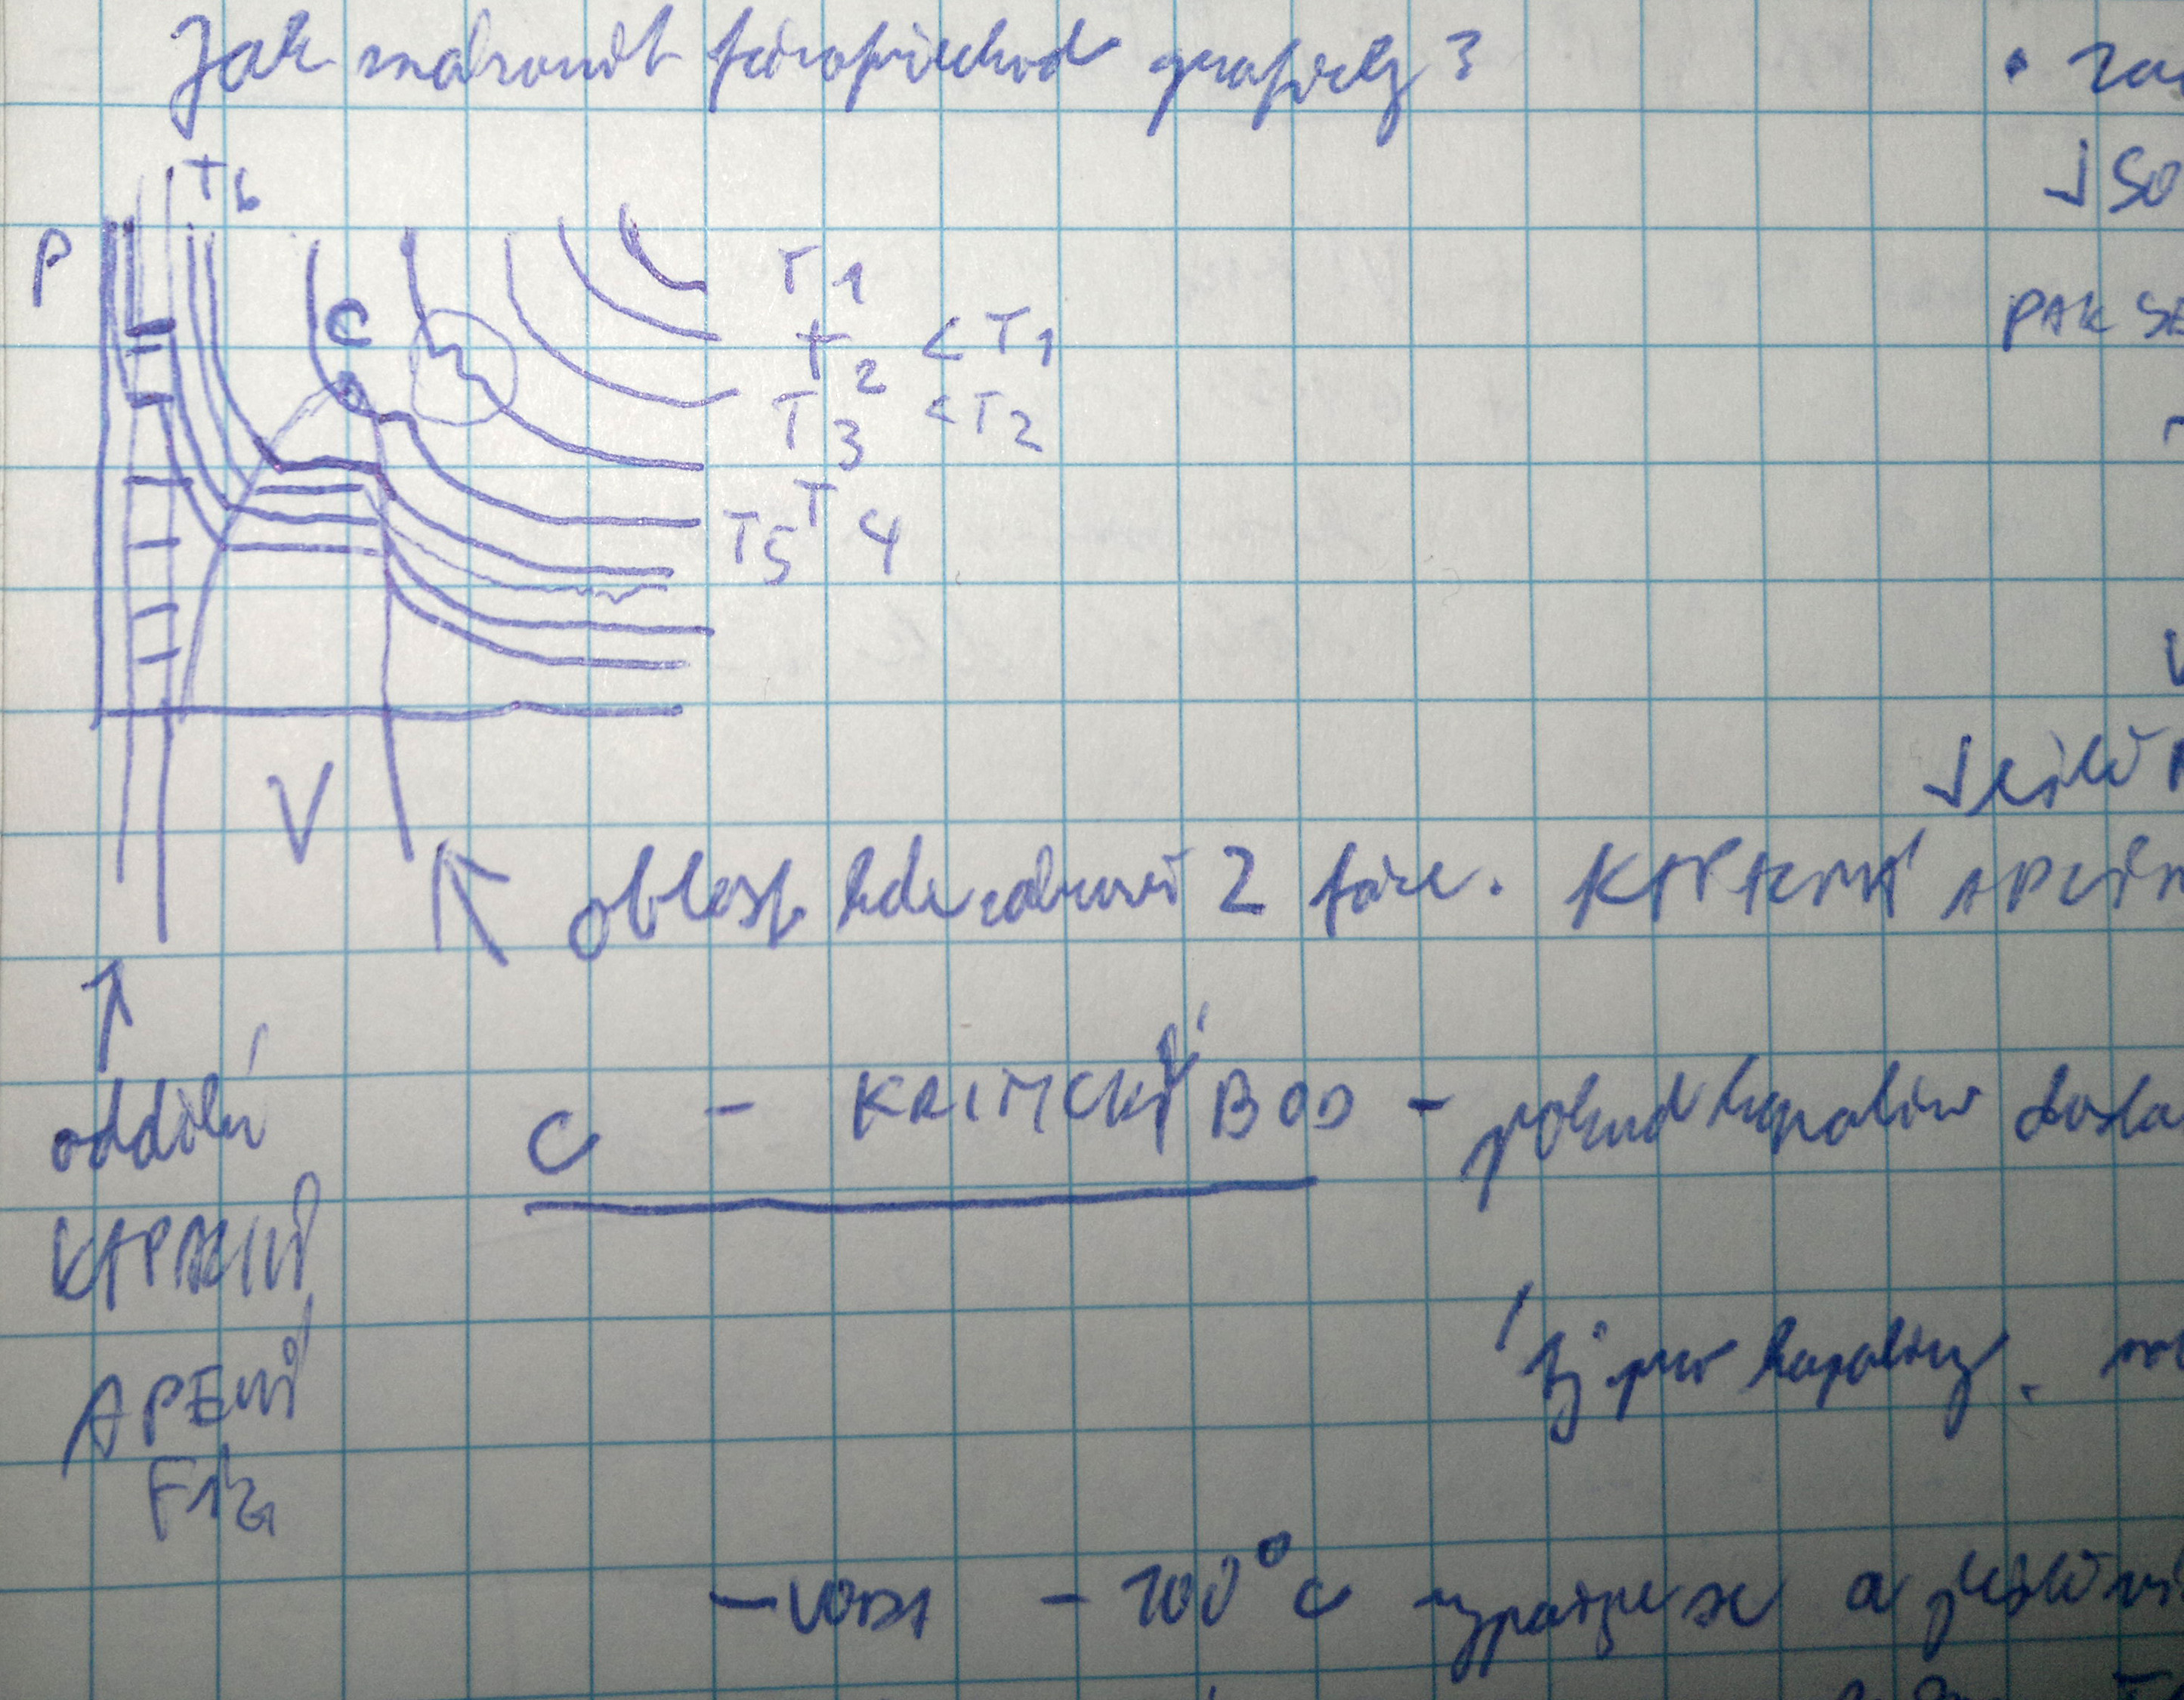
\includegraphics[width=0.4\textwidth]{2014-03-30-1595}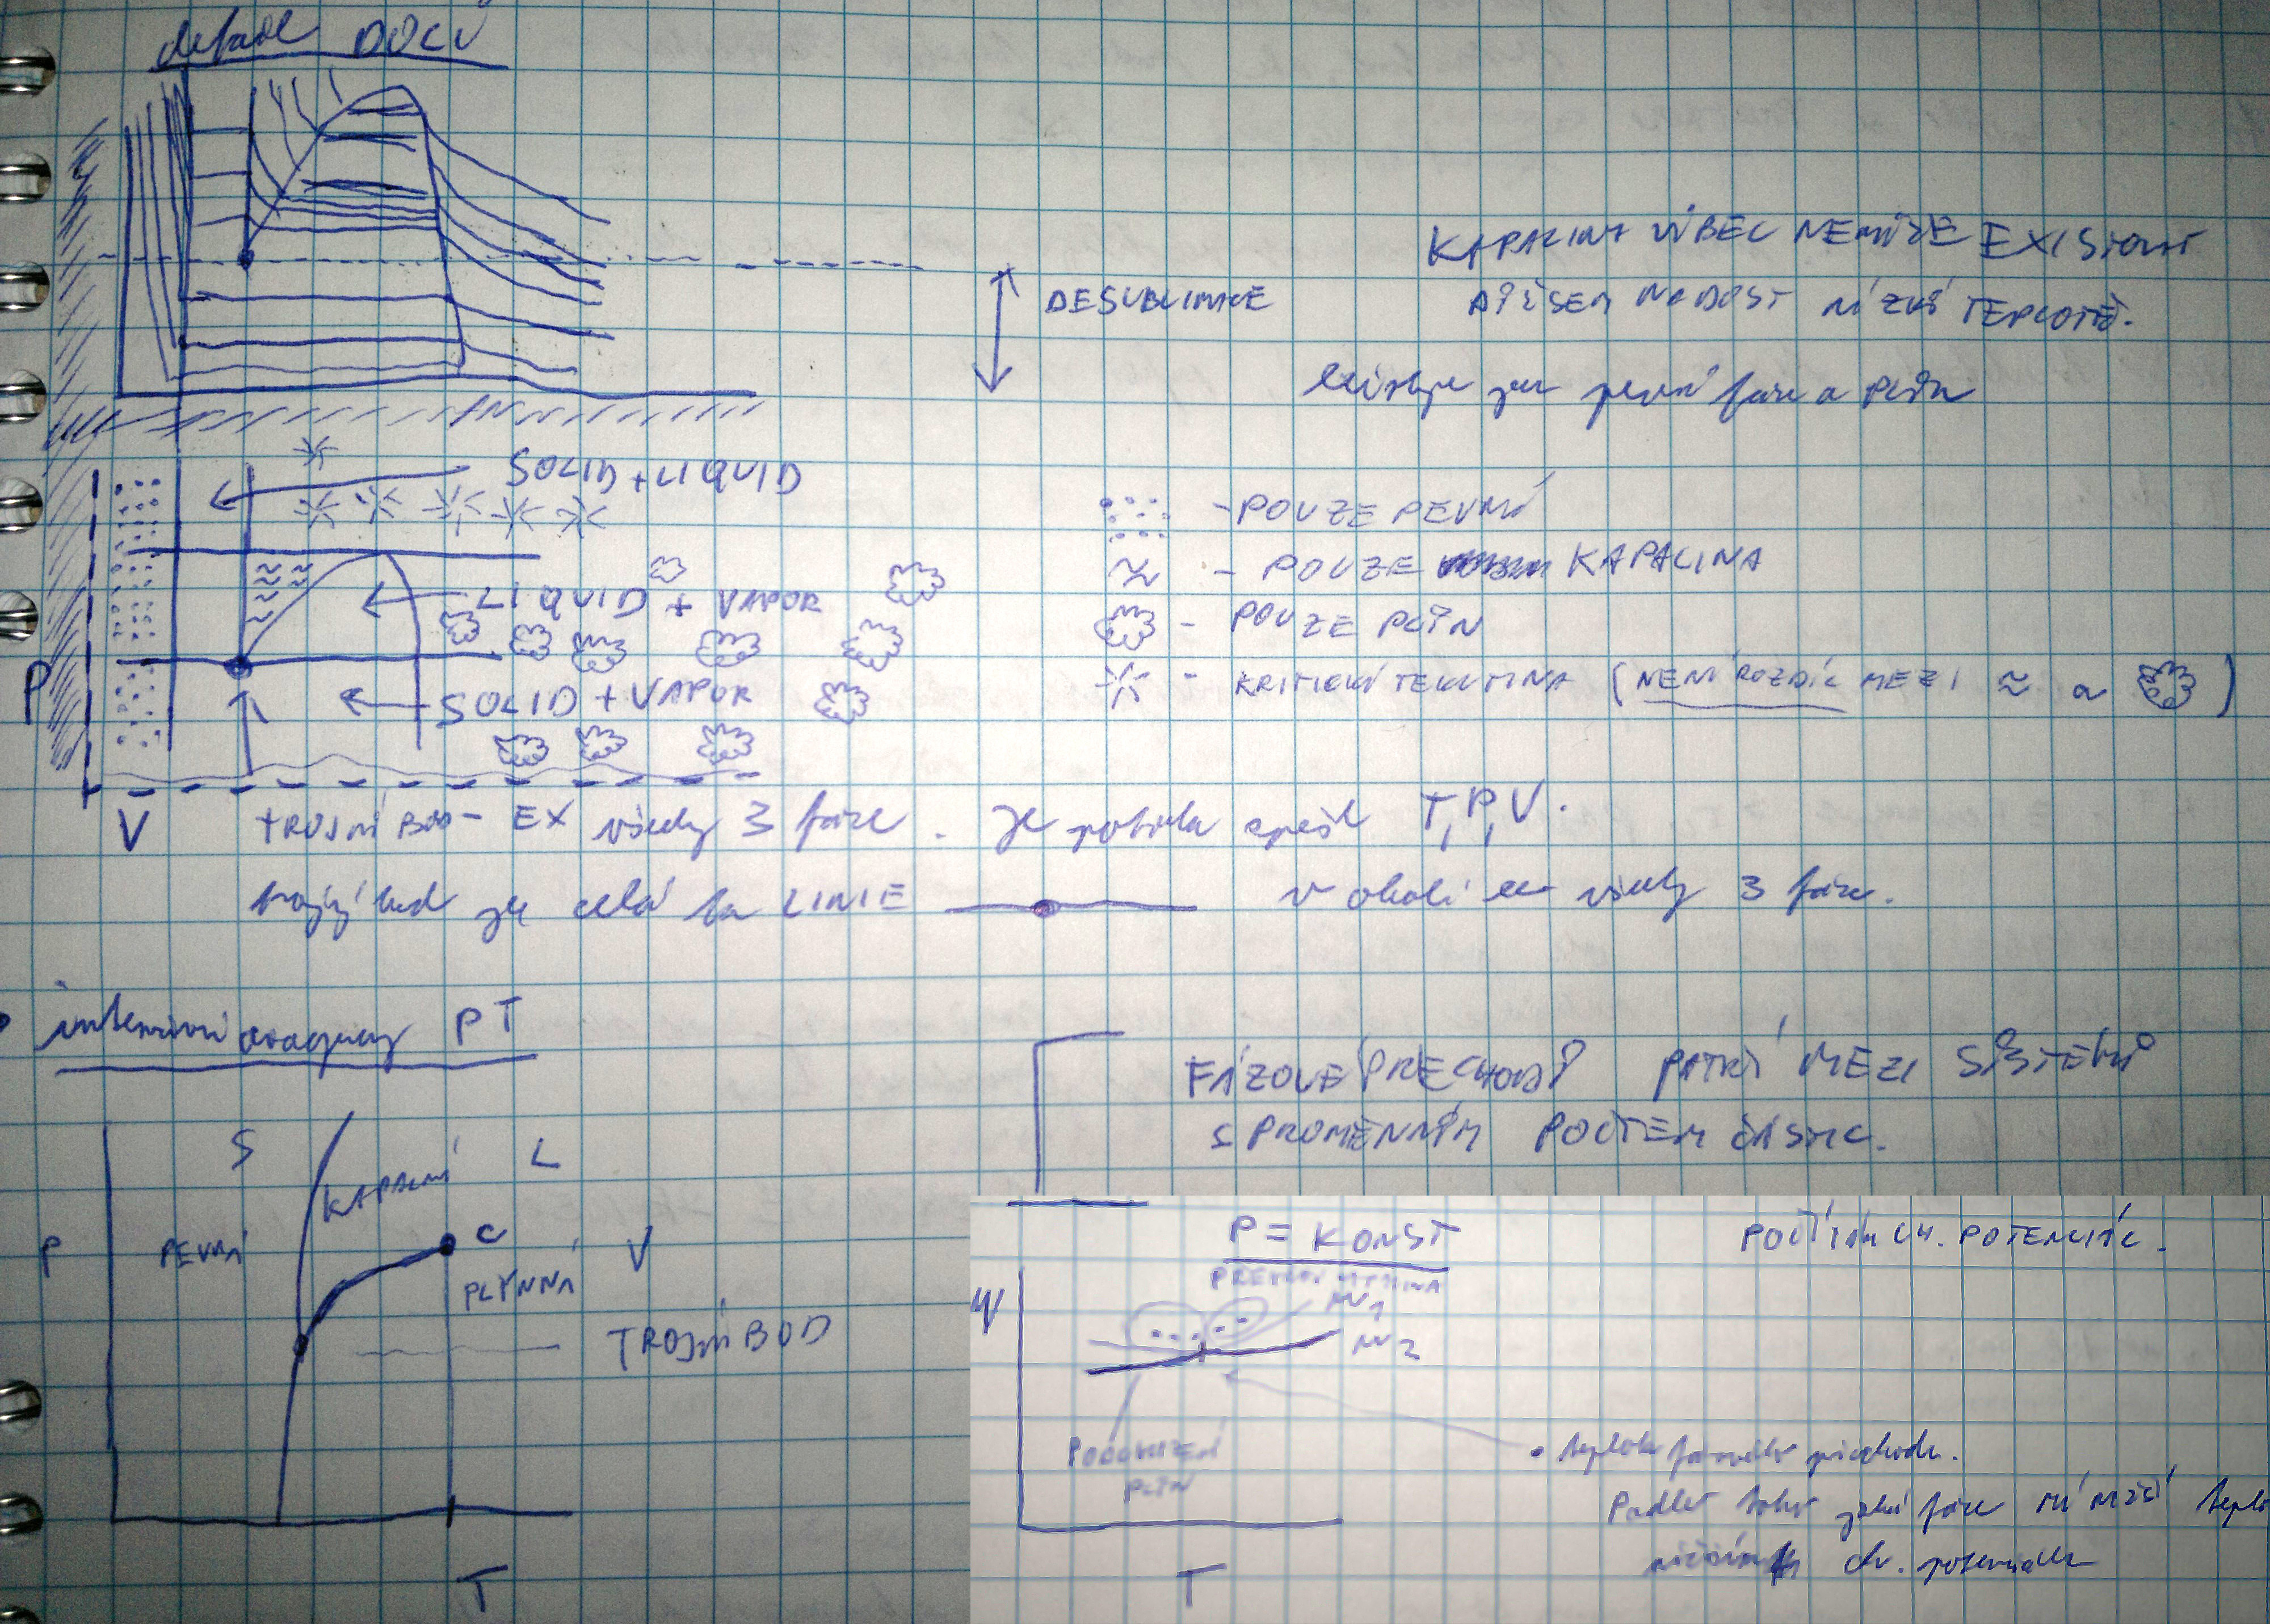
\includegraphics[width=0.6\textwidth]{2014-03-30-1598}

\end{figure}


K fázovému přechodu je potřeba vytvořit fázové rozhraní. To vyžaduje
spoustu energie, pokud tam už náhodou není. Pokud není, tak zůstává
ve fázi energeticky nevýhodný - metastabilní stav.

Metastabilní stav čeká na fluktuaci (např. přesycená pára). Nebo na
kondenzační zárodky. Proto funguje mj. i bublinková mlžná komora.

Trojný bod - podmínka (na teplotu), kdy můžou existovat všechny tři
fáze.


\paragraph*{Vícesložkové systémy a fázové přechody}


\paragraph*{Gibbsovo fázové pravidlo}

Mějme systém tvořený $n$ složkami/komponentami nacházející se v $r$
fázích. Kolik fází maximálně se může najednou vyskytovat?

Vyskytuje li se systém v $r$ fázích najednou, musí se rovnat chemické
potenciály pro každou komponentu. 

To je $n(r-1)$ rovnic, musíme mít dost volných parametrů systému,
co mi umožní tohle nezávisle ladit. Kolik je těch parametrů - $\mu_{n}^{(r)}(T,p,c_{1}^{(r)}...c_{n-1}^{(r)})$
-

\[
\mu_{1}^{(1)}=...=\mu_{1}^{(r)}
\]


\[
...
\]


\[
\mu_{n}^{(1)}=...=\mu_{n}^{(r)}
\]


...celkem $2+r(n-1)$ vs $n(r-1)$ rovnic, řešitelné pokud proměnných
víc než rovnic, tedy $2+n\geq r$.

Pozn. Eutektický diagram, fázový diagram binárního systému. Pomocí
linií fázových přechodů je možné čistit směsi.


\paragraph*{Rychlost šíření zvuku v plynu}

Předpokládáme li slabý zvuk (malé výchylky), nemalý tlak, pak lze
z vlnové rovnice dostat $c=\frac{\kappa k_{B}T}{M}$. Kappa je konstanta
z adiabatického děje, $M$ hmotnost jedné částice.


\paragraph*{Přímou integrací z rozdělení odvodit stavovou rovnici ideálního plynu}

Rozdělení které použijeme bude Maxwell-Boltzmannovo (pro hybnosti,
resp. polohy):

\[
p_{MB}(p,r)=p_{M}(p)\cdot p_{B}(r)
\]


Maxwellovo rozdělení je hustota pravděpodobnosti, že změřím částice
s hybností $p$ (a jako počet částic v nějakém objemu vezmeme $p_{B}=N/V$).

\[
p_{M}(\vec{p})=(2\pi mk_{B}T)^{-3/2}\exp(\frac{-p^{2}}{2mk_{B}T})
\]


Tohle rozdělení použijeme k dosazení dále. Hlavní fyzikální úvaha
je nicméně následující:

Tlak na hranici (kolmé na směr $x$) jistého objemu je daný silou
narážejících částic impulzem síly $2p_{x}=F\delta t$. Jaké částice
tam můžou přiletět? Jen ty co to stihnou za $\delta t$ a jen ty co
se nacházejí v objemu daném plochou $S$ a výškou $v_{x}=p_{x}/m$.
Fluktuace bereme, že se ve střední hodnotě vyruší a protože je plyn
homogenní, tak částice co přiletí šíkmo jsou započítány také (za každou
co přiletí šikmo odjinud do objemu jedna vyletí šikmo z objemu jinam).

Vezmeme tedy hranici kolmou na směr $x$, o ploše $S$, síla je dána
takto:

\[
PS=\frac{p_{x}}{m}
\]


...doadíme úvahu o částicích způsobujících impuls síly (s pomocí vztahu
pro impulz síly):

\[
PS=\iiint_{\begin{array}{c}
p_{x}\geq0\\
p_{y,p_{z}\in\mathbb{R}}
\end{array}}\frac{Sv_{x}\delta t}{V}\frac{2p_{x}}{\delta t}p_{M}(p)\, dp_{x}\, dp_{y}\, dp_{z}=
\]


...první zlomek vyjadřuje jestli se částice nachází v dané části objemu
kde může do stěny narazit, druhý zlomek vyjadřuje sílu (hybnost dělená
časem - díky tomu se $\delta t$ vykrátí) a $p_{M}$ je maxwellovo
rozdělení hybností. Po vyintegrování dostaneme:

\[
=\frac{2SN\sqrt{\pi}}{4Vm\sqrt{2\pi mk_{B}T}}(2mk_{B}T)^{3/2}=S\frac{k_{B}T}{V}
\]


...což po vykrácení $S$ dá:

\[
PV=Nk_{B}T
\]



\paragraph*{Chemický potenciál ideálního plynu}

\[
\mu=k_{B}T\ln(\frac{N}{V}(\frac{2\pi\hbar^{2}}{mk_{B}T})^{3/2})
\]



\paragraph*{Raoultův zákon}

Mikroskopický zákon o celkovém tlaku jako součtu tlaků složek násobeno
koncentrací:

\[
p=\sum_{i}p_{i}x_{i}
\]



\paragraph*{Duhem-margules rovnice}

\[
\sum_{s}x_{s}d(\ln P_{S})=0
\]



\paragraph*{Osmotický tlak}

\[
\mathbb{T}=\frac{-k_{B}T}{v}\ln x_{1}
\]


Závisí na logaritmu složení.


\section*{Poznámky}


\paragraph*{GIT}

\url{https://github.com/Darthholi/TermodynStatFyz}

Pokud nemáte účet na GIThubu a chcete poznámky editovat, budu mít
jen radost, pokud mi zašlete novou verzi na \textit{mholecek91@volny.cz.}
\end{document}
